\renewcommand{\myepsfbox}[1]{\epsfbox{appD/#1}}

\newpage
\onecolumn
\chapter{参考資料}

TeCをもっと活用してもらうために,
拡張ボード,TeCの回路図,FPGAのピン配置表等を掲載します.
次のページから以下の資料を掲載します.

\subsubsection{TeC7基板回路図}
TeC7本体のプリント基板回路図です.

\subsubsection{TeC7ピン配置表}
TeC7に搭載されているXilinx Spartan-6 FPGA (XC6LX9-2TQG144C)の
ピンがどのように利用されているか示す一覧表です.

\newpage
\begin{figure*}[btph]
\begin{center}
%\includegraphics[angle=90,clip, bb=0 0 842 595, width=12cm]
%\includegraphics[angle=90,clip, bb=20 25 822 525, width=14cm]
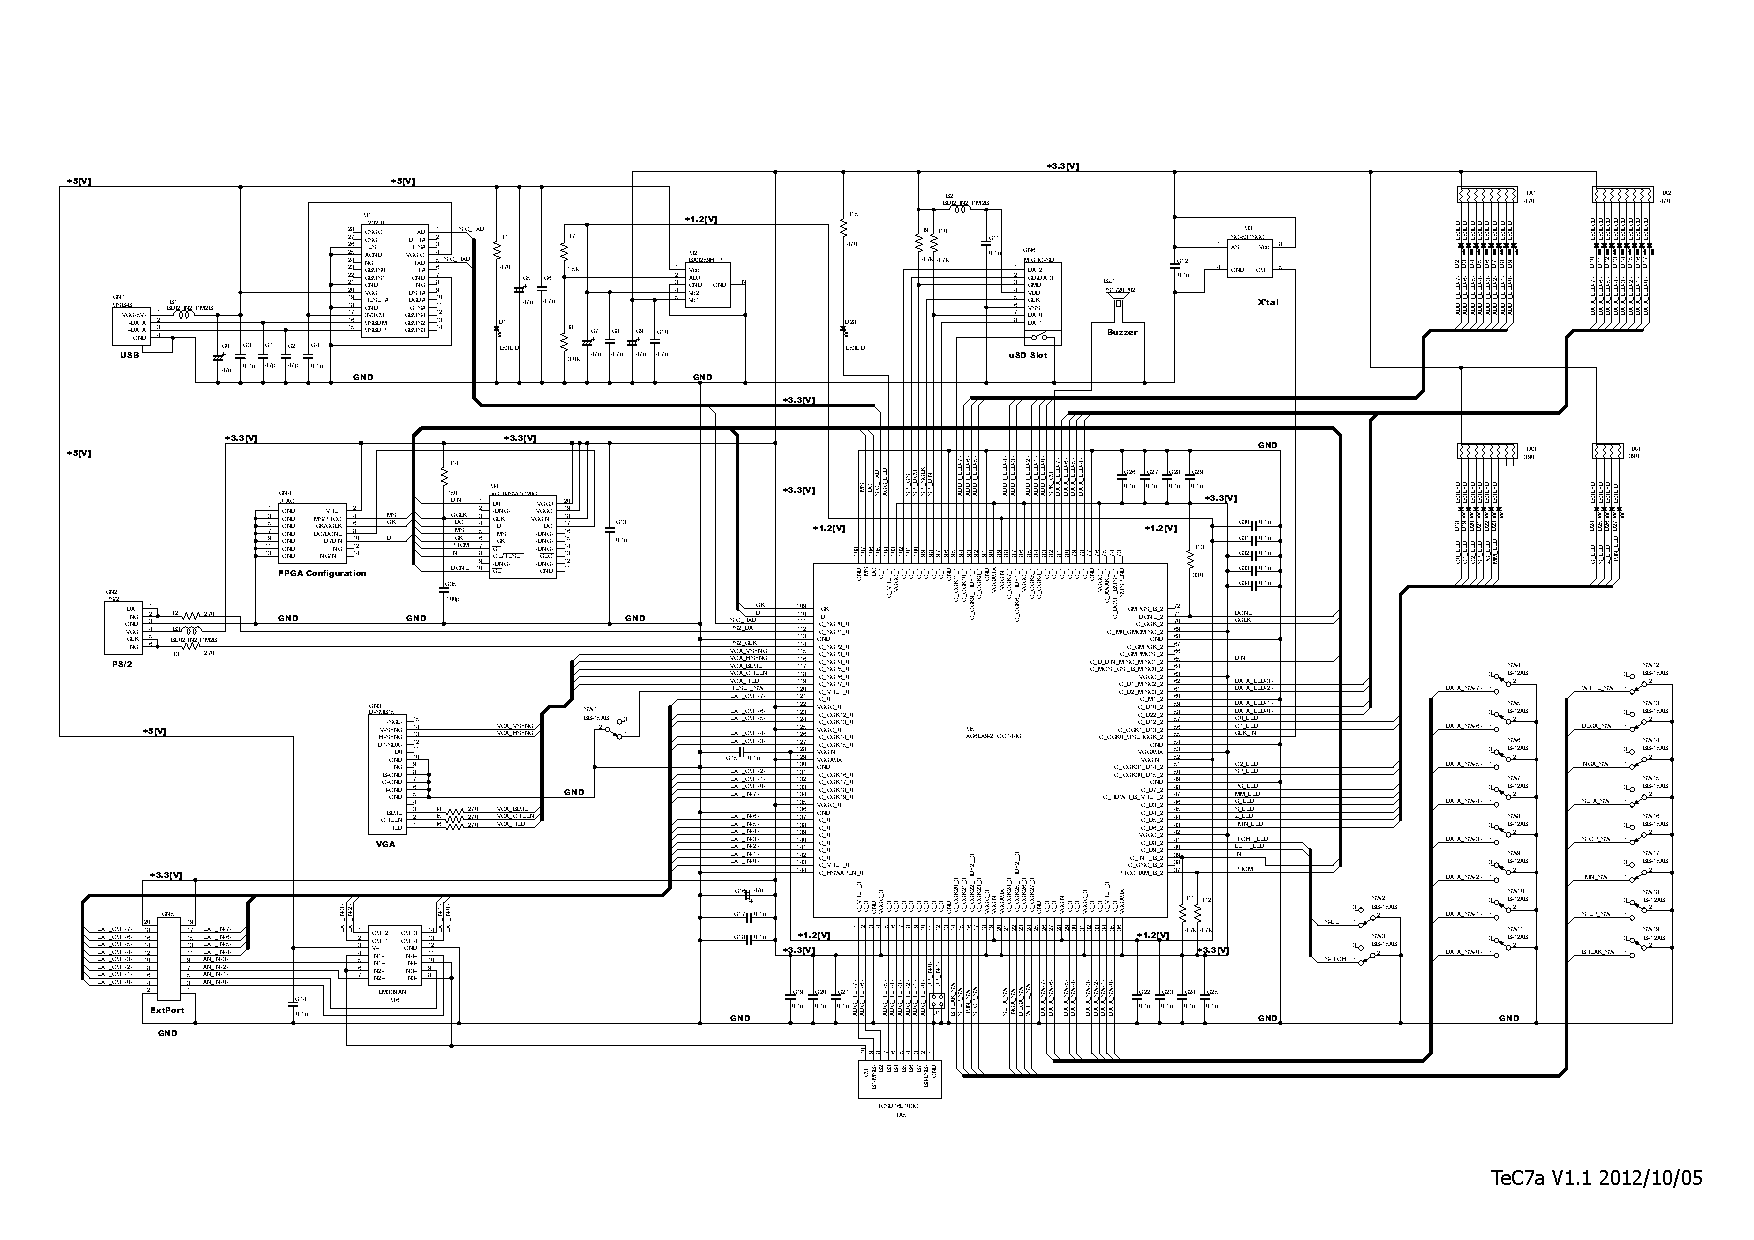
\includegraphics[angle=90,width=14cm]
{appD/TeC7a.pdf}
\caption{TeC7基板回路図}
\end{center}
\end{figure*}

\newpage
\begin{figure*}[btph]
\begin{center}
%\includegraphics[angle=90,clip, bb=50 120 792 545, width=13cm]
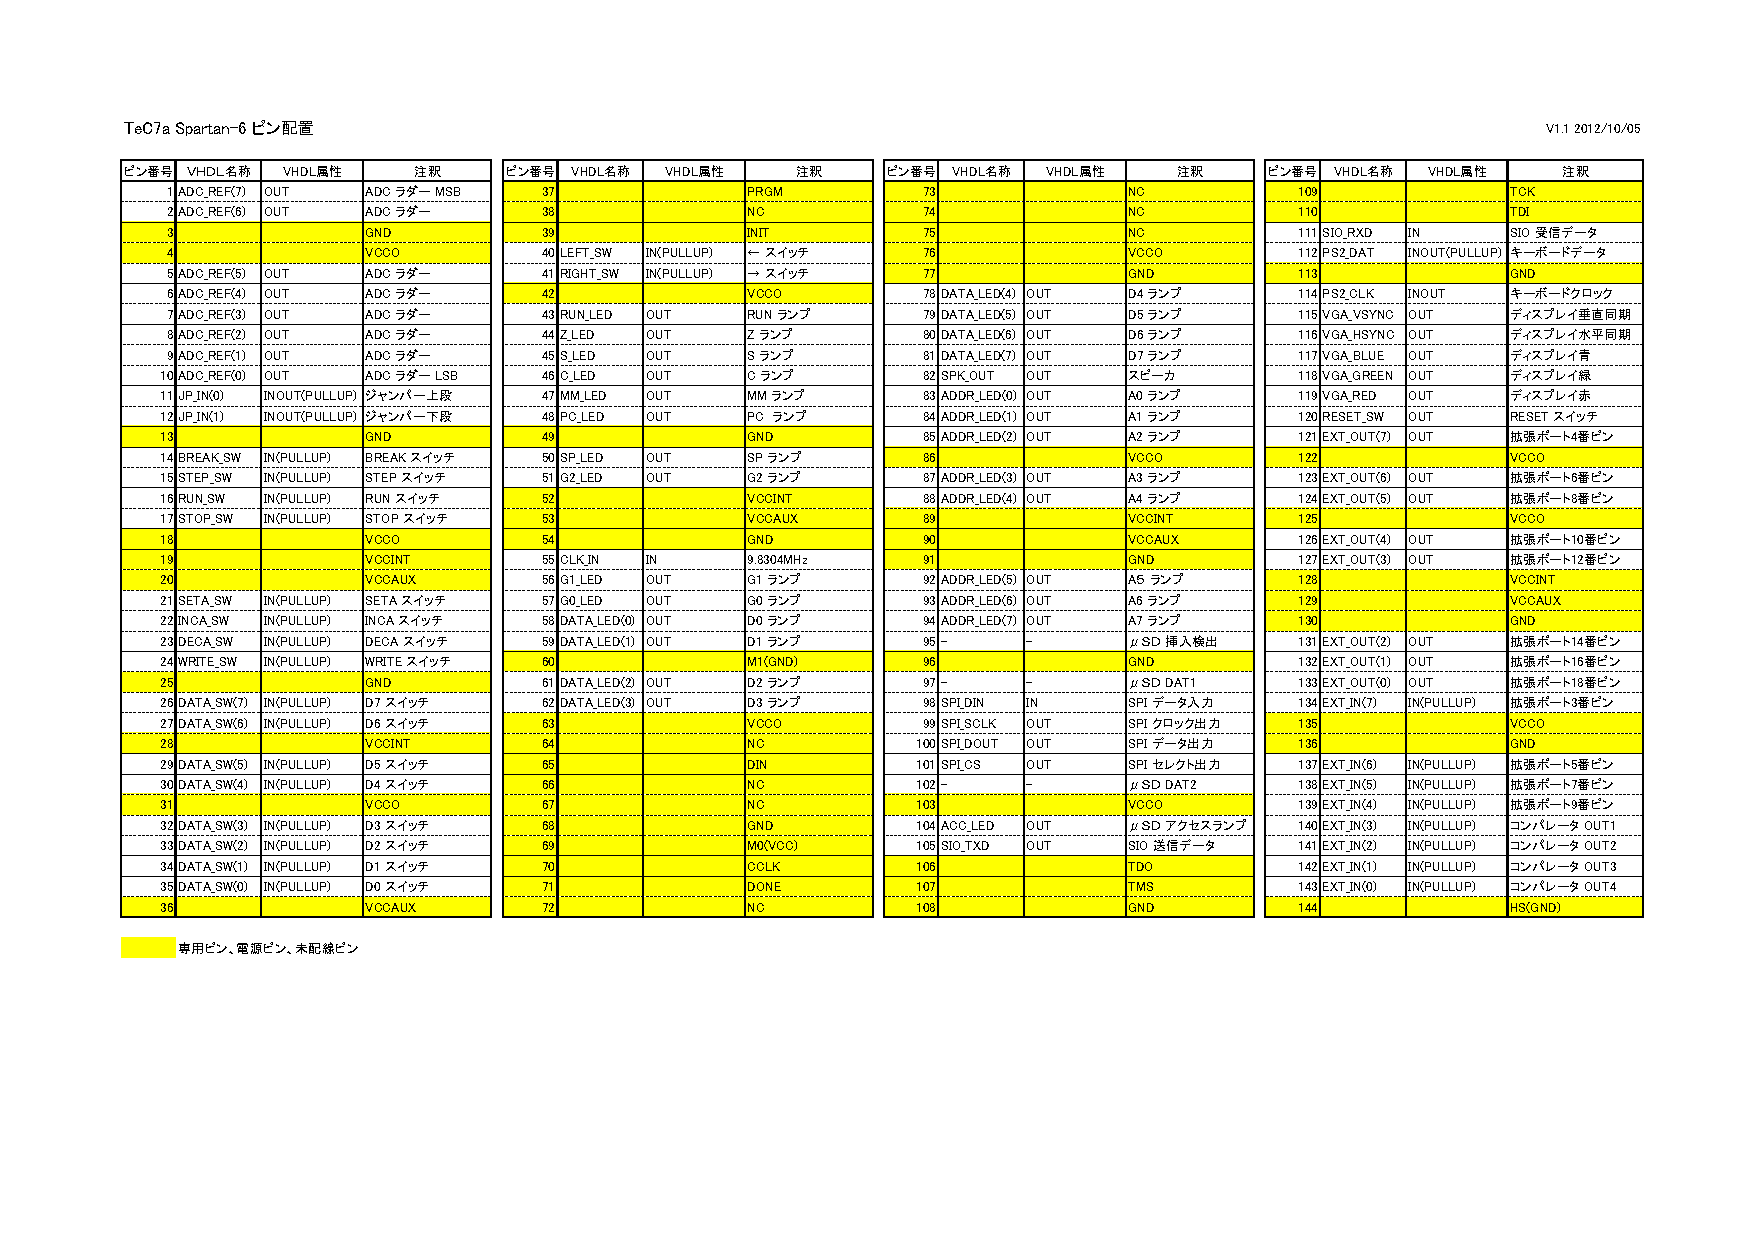
\includegraphics[angle=90, width=12.5cm]
{appD/TeC7aPIN.pdf}
\caption{TeC7ピン配置図}
\end{center}
\end{figure*}

%\includegraphics[angle=90,bb=100 100 横ピクセル数 縦ピクセル数,width=16.8]{ファイル名}

